% \section{Logical view: components}
% \label{sec:Components}

%
% This is the merging of "component view" and "component interafctions"
% from J&M outline, following Saba's suggestion.
%

To provide the best solutions for LAr TPC simulation, reconstruction and
analysis of data, LArSoft interacts with other software aimed to
provide developers with tools commonly in use by the broader physics community,
standardize code development,
and allow for experiment-specific needs (\cref{fig:LArSoftRelations}).
\begin{figure}
   \centering
   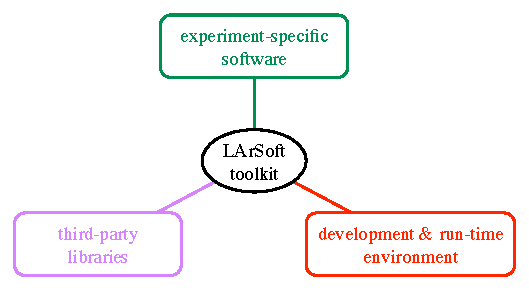
\includegraphics{figures/LArSoftEnvironmentOverview}
   \caption{\label{fig:LArSoftRelations}
      Relationship of LArSoft with other software categories.
   }
\end{figure}

Physics developers typically rely on copious libraries providing general or physics-specific services
(\cref{fig:LArSoftRelations:Libraries}).
LArSoft already offers:
\begin{itemize}
   \item access to a framework, \ART~\cite{ART}, providing essential functionalities
      including an event data model, an event loop, workflow definition and control,
      plug-in of code, distribution and tracking of job configuration,
      serialization of the results, and more
   \item proxy-, web-based access to data bases via \libwda~\cite{libwda},
      or direct access to \PostgreSQL databases\footnote{%
      Experience has shown that direct database does not scale well with the number of accessing jobs.%
      }
   \item physics libraries, as CERN \CLHEP~\cite{CLHEP} and \nutools~\cite{nutools}
   \item event generation packages: \GENIE~\cite{GENIE}, \CRY~\cite{CRY}, HEPEVT~\cite{HEPEVT} files
   \item detector simulation libraries (to date, only GEANT4~\cite{GEANT})
   \item pattern recognition libraries, like \Pandora
   \item data analysis tools, like CERN \ROOT~\cite{ROOT}
   \item visualization aids, also with CERN \ROOT and \nutools
\end{itemize}
Additional libraries are expected to be added in the future.
\begin{figure}
   \centering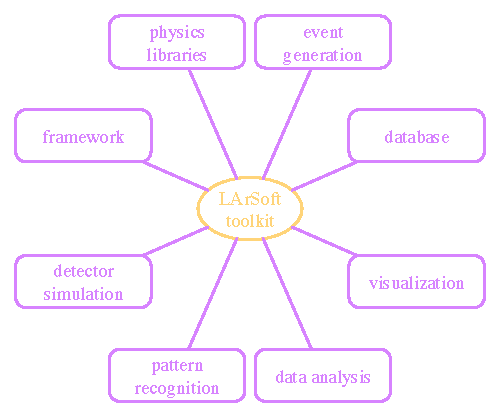
\includegraphics{figures/LArSoftThirdPartyLibraries}
   \caption{\label{fig:LArSoftRelations:Libraries}
      Relationship between LArSoft and third-party libraries.
   }
\end{figure}
\begin{figure}
   \centering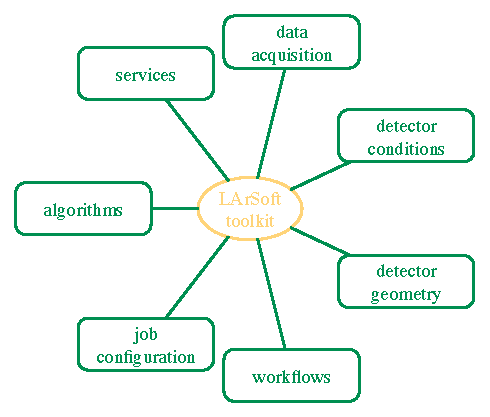
\includegraphics{figures/LArSoftExperimentSoftware}
   \caption{\label{fig:LArSoftRelations:Experiments}
      Relationship between LArSoft and experiment-specific software.
   }
\end{figure}

LArSoft is designed to accommodate specific needs from the experiments.
Experiments directly contribute LArSoft content when it's suitable,
\ie when of general utility and experiment-agnostic.
In the other cases, experiments interface to LArSoft though many channels
(\cref{fig:LArSoftRelations:Experiments}):
\begin{itemize}
   \item detector geometry is provided in GDML or ROOT format
   \item detector conditions can be learned via static configuration or from experiment databases
   \item detector data is acquired by special \ART modules or by standard \ART files (e.g., produced by \ARTDAQ) containing standard LArSoft data products
   \item specialized services and algorithms can be plugged in using the \ART framework
   \item job configuration, controlling the data to be processed and the sequence of actions to perform,
      is specified in \FHiCL language~\cite{FHiCL}
   \item workflows are defined by the experiment, typically by using custom scripts that include the execution of LArSoft main program, \texttt{lar}
\end{itemize}
\begin{figure}
   \centering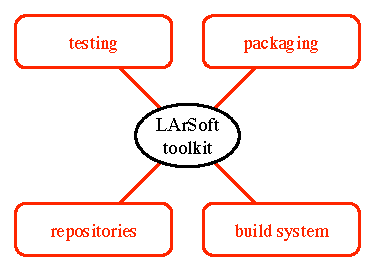
\includegraphics{figures/LArSoftDevelopmentRunTime}
   \caption{\label{fig:LArSoftRelations:Development}
      Relationship between LArSoft and development software categories.
   }
\end{figure}

LArSoft has a large number of interdependent components,
and provides the users tools to facilitate code development (\cref{fig:LArSoftRelations:Development}).
LArSoft code is organized in repositories that can be compiled when needed.
The building system ensures consistent builds among all supported platforms.
The \UPS~\cite{UPS} distribution system ensures that the same consistency is preserved at run time.
Infrastructure for automatic execution of user tests is also provided,
together with a growing number of tests exercising parts of LArSoft tools.



\subsection{Internal components}
\label{ssec:Components}

Most LArSoft components can be grouped into some broad functional categories.
Some of them are well established, while others are being developed now or have been just designed.
The following list touches the main ones, without being exhaustive:
% \begin{itemize}
%    \item physical constants
%    \item helpers for common framework usage patterns (\eg, creation of asociations between data products)
%    \item detector geometry description
%    \item persistent data structures (``data products'')
%    \item detector information services: liquid argon and detector properties, detector clocks, readout channel quality
%    \item calibration services: readout channel pedestals
%    \item physics event generation
%    \item detector simulation: TPC and optical detectors
%    \item readout simulation: template modules for TPC and optical detectors
%    \item simulation of optical triggers
%    \item calibration: template modules, description of residual electric charge in TPC volume
%    \item object reconstruction: 1D (TPC wire hits, optical hits), 2D (TPC hit clusters), 3D (tracks, showers, vertices) and time (optical flashes)
%    \item TPC hit simulation and correlation between reconstructed objects and generated particles
%    \item energy and momentum reconstruction (``calorimetry'')
%    \item particle identification
%    \item global event reconstruction
%    \item graphical display of generated and reconstructed objects (``event display'')
%    \item analyser module example
% \end{itemize}
\begin{description}
   \item[detector information] \mbox{} % make it start a new line
      \begin{itemize}
         \item detector geometry description
         \item detector information services: liquid argon and detector properties, readout timings and settings, readout channel quality
         \item calibration services: readout channel pedestals
         \item map of residual electric charge in TPC volume
      \end{itemize}
   \item[persistent data structures] (``data products''), grouped in
      \begin{itemize}
         \item raw data, unprocessed from the detector
         \item simulation from event generator (``truth'') and detector simulation
         \item reconstruction of detector and physics objects
         \item optical data, raw or processed, from the optical detectors
         \item analysis results of reconstructed objects
      \end{itemize}
   \item[operations] \mbox{} % make it start a new line
      \begin{itemize}
         \item physics event generation
         \item detector simulation: TPC and optical detectors
         \item readout simulation: template modules for TPC and optical detectors
         \item simulation of optical triggers
         \item calibration template modules
         \item object reconstruction: 1D (TPC wire hits, optical hits), 2D (TPC hit clusters), 3D (tracks, showers, vertices) and time (optical flashes)
         \item TPC hit simulation and correlation between reconstructed objects and generated particles
         \item energy and momentum reconstruction (``calorimetry'')
         \item particle identification
         \item global event reconstruction
      \end{itemize}
   \item[programming utilities] and framework interface
      \begin{itemize}
         \item physical constants
         \item helpers for common framework usage patterns (\eg, creation of asociations between data products)
      \end{itemize}
   \item[graphical display] of generated and reconstructed objects (``event display'')
   \item[example] of analysis module
\end{description}
